\documentclass[10pt]{beamer}

\usepackage[english]{babel}
\usepackage[utf8]{inputenc}
\usepackage{amssymb}
\usepackage{amsthm}
\usepackage[all]{xy}
\usepackage{graphicx}

%% Stuff
\renewcommand{\le}{\leqslant}
\renewcommand{\ge}{\geqslant}  % comme François le demande...
\newcommand{\blue}[1]{\textcolor{blue}{#1}}  % colouring
%% Algèbre
\newcommand{\clot}[1]{\bar{#1}}  % clôture algèbrique
\newcommand{\card}[1]{\# #1}  % cardinalité d'un ensemble
\DeclareMathOperator{\car}{char}  % caractéristique d'un corps
\DeclareMathOperator{\Frac}{Frac}  % corps des fractions
\newcommand{\Z}{\mathbb{Z}}  % les entiers
\newcommand{\K}{\mathbb{K}}  % un corps
\newcommand{\LK}{\mathbb{L}}  % encore un corps
\newcommand{\U}{\mathbb{U}}  % encore un corps
\newcommand{\F}{\mathbb{F}}  % un corps fini
\newcommand{\Q}{\mathbb{Q}}  % les rationnels
\newcommand{\R}{\mathbb{R}}  % les réels
\newcommand{\C}{\mathbb{C}}  % les complexes
\newcommand{\isom}{\cong}  % isomorphisme de corps
\newcommand{\frob}{\varphi}  % fröbenius
\DeclareMathOperator{\Gal}{Gal}  % groupe de Galois
\DeclareMathOperator{\Tr}{Tr}  % trace
\DeclareMathOperator{\PTr}{PTr}  % pseudotrace
\DeclareMathOperator{\Norm}{N} % norme
\newcommand{\euler}{\phi}  % indicatrice d'Euler
\DeclareMathOperator{\ord}{ord}  % l'ordre d'un élément
\newcommand{\AS}[1]{\mathcal{#1}}  % la police des polynômes d'AS
\DeclareMathOperator{\rev}{rev}  % le reverse d'un polynôme
%% Courbes
\DeclareMathOperator{\Jac}{Jac}  % la jacobienne
\newcommand{\Proj}{\mathbb{P}}  % espace projectif
\newcommand{\0}{\mathcal{O}}  % point de base d'une courbe
\newcommand{\ecpoint}[3]{[#1:#2:#3]}  % un point d'une courbe
\newcommand{\isog}[1]{\mathcal{#1}}  % la police des isogénies
\newcommand{\I}{\isog{I}}  % une isogénie I
\newcommand{\Hasse}{H}  % l'invariant de Hasse
\newcommand{\divpol}{f}  % polynôme de division
%% Autre
\newcommand{\tildO}{\tilde{O}}  % la notation O~ qui oublie les log
\newcommand{\Mint}{\mathrm{\sf M}_\text{int}}  % fonction de multiplication
\newcommand{\Mpol}[1][]{\mathrm{\sf M}_\text{pol}^{#1}}  % fonction de multiplication
\newcommand{\Mult}[1][]{\mathrm{\sf M}_{#1}}  % fonction de multiplication
\newcommand{\Push}{\mathrm{\sf P}}  % fonction de push-down
\newcommand{\Lift}{\mathrm{\sf L}}  % fonction de lift-up
\newcommand{\Trace}{\mathrm{\sf T}}  % fonction de trace
\newcommand{\Frob}{\mathrm{\sf F}}  % fonction de frobenius itéré
\newcommand{\Ptr}{\mathrm{\sf PT}}  % fonction de pseudo-trace
\newcommand{\ModComp}{\mathrm{\sf C}}  % fonction de composition modulaire
\newcommand{\alg}[1]{\textsf{#1}}  % la police des algorithmes
\newcommand{\wrt}{\dashv}  % appartenance forte, a\wrt A signifie que a est représenté comme un élément de A
\DeclareMathOperator{\op}{op}  % une opération

\newenvironment{algorithm}[3]{\begin{center}\begin{minipage}{0.85\textwidth}
      \sf
      \rule{\textwidth}{0.2pt}\\
      \makebox[\textwidth][c]{\textbf{#1}}\\
      \rule[0.5\baselineskip]{\textwidth}{0.2pt}\\
      \textbf{Input~~} #2\\
      \textbf{Output} #3
      \smallskip
      \begin{enumerate}
}{\end{enumerate}
      \rule{\textwidth}{0.2pt}
\end{minipage}\end{center}}

% beamer-specific
%\setbeamertemplate{theorem begin}{
%  \begin{\inserttheoremblockenv}{
%      Théorème
%      \ifthenelse{\equal{\inserttheoremaddition}{}}
%		 {}
%		 {(\inserttheoremaddition)}    
		 %  \ifx\inserttheoremaddition\@empty\else\ (\inserttheoremaddition)\fi
%    }
%}

\mode<presentation>{%
  \usetheme[]{Madrid}
  \usefonttheme[onlymath]{serif}
  \usecolortheme{seahorse}
  \usecolortheme{rose}
}


\title{Computing isogenies in small characteristics}
\author[L.~De~Feo]{L.~De~Feo}
\institute[TANC, LIX]{Projet TANC, LIX, École Polytechnique, Paris, France}
\date[Bordeaux, June 19, 2009]{June 19, 2009\\Université de Bordeaux 1}


%% \AtBeginSection[]
%% {
%%   \begin{frame}<beamer>
%%     \frametitle{Plan}
%%     \tableofcontents[currentsection]
%%   \end{frame}
%% }


\begin{document}

\begin{frame}
  \titlepage
\end{frame}

%%
%%

\section{Introduction}

\begin{frame}
  \frametitle{Elliptic curves}

  \begin{columns} 
    \begin{column}{0.55\textwidth}
      \begin{block}{Elliptic curves}
        \begin{itemize}
        \item (Finite) field $\K$, with closure $\clot{\K}$,
        \item Weierstrass form: let $a,b\in\K$, 
          \[E \;:\; Y^2 = X^3 + aX + b\]
        \item $E(\K)$ set of $\K$-rational points,
        \item $E(\K)$ is a (finite) group. May be used for crypto.
        \end{itemize}
      \end{block}

      \begin{block}{$j$-invariant}
        \[j(E) = \frac{1728(4a)^3}{16(4a^3 + 27b^2)}\]
        Two elliptic curves are isomorphic over $\clot{\K}$ iff they
        have the same $j$-invariant.
      \end{block}
  
    \end{column}

    \begin{column}{0.4\textwidth}
      \begin{figure}
        \centering
        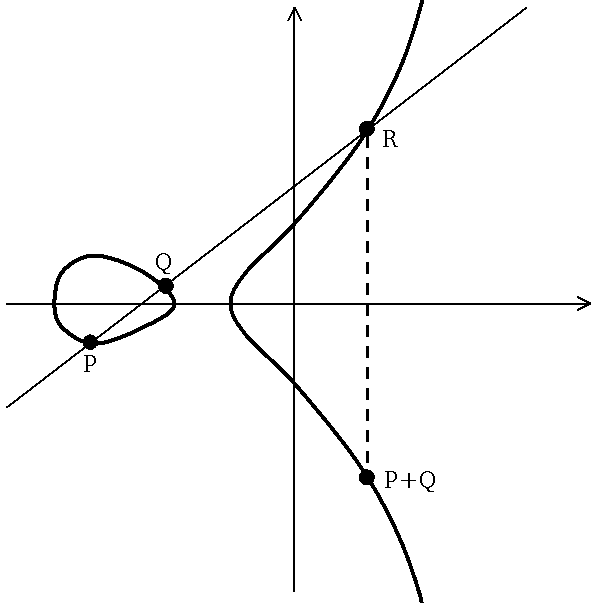
\includegraphics[width=\textwidth]{ecadd}
        \caption{point addition on a Weierstrass curve over $\R$}
      \end{figure}
    \end{column}
  \end{columns}
\end{frame}

%%

\begin{frame}
  \frametitle{Isogenies}

  \frametitle{Isogenies}
  
  \centering $\xymatrix{ E(\clot{\K}) \ar[r]^\I & E'(\clot{\K})}$

  \begin{block}{Isogeny}
    \begin{itemize}
    \item Rational map: $\qquad \I(X,Y) =
      \left(\frac{a(X,Y)}{b(X,Y)},\frac{c(X,Y)}{d(X,Y)} \right)$,
    \item onto, finite kernel, $\qquad\deg\I = [\clot{\K}(E'):\I^\ast
      \clot{\K}(E)]$,
    \item group morphism: $\qquad \I(P+Q) = \I(P) + \I(Q),\quad \I(\0_E)
      = \0_{E'}$
    \end{itemize}
  \end{block}

  \begin{block}{Examples}
    \begin{overprint}
      \onslide<1>
      Multiplication
      \begin{align*}
	[m] : E(\clot{\K}) &\rightarrow E(\clot{\K})\\
	                   P &\mapsto [m]P
      \end{align*}
      $\;\deg [m] = m^2$, $\;\ker\I = E[m]$.

      \onslide<2|handout:0>
      \emph{Small} Frobenius map
      \begin{align*}
	\frob_p : E(\clot{\K}) &\rightarrow E^{(p)}(\clot{\K})\\
	                   (X,Y) &\mapsto (X^p,Y^p)
      \end{align*}
      where $\;\;E^{(p)} \;:\; Y^2 = X^3 + a^pX + b^p\qquad$ if $p =
      \car(\K)$,\\
      $\;\deg \frob_p = p$, $\;\ker\frob_p = \{\0\}$.
 
      \onslide<3|handout:0>
      Frobenius endomorphism
      \begin{align*}
	\frob_q : E(\clot{\K}) &\rightarrow E(\clot{\K})\\
	                   (X,Y) &\mapsto (X^q,Y^q)
      \end{align*}
      if $\K = \F_q$ then $E^{(q)} = E$, $\;\deg \frob_q = q$,
      $\;\ker\frob_q = \{\0\}$.

      \onslide<4|handout:0>
      Separable isogenies
      \[\quad\I(X,Y) = \left(\frac{g(X)}{h^2(X)},
      cY\left(\frac{g(X)}{h^2(X)}\right)'\right)\] $\;\deg\I =
      \card{\ker\I} \approx \deg h$.
    \end{overprint}
  \end{block}
\end{frame}

%%

\begin{frame}
  \frametitle{Dual isogeny}

  \[\xymatrix{
    E \ar[r]^\I \ar[dr]_{[m]} & E'\ar[d]^{\hat\I}\\
    & E
  }\]

  \begin{theorem}[Dual isogeny]
    $\I$ of degree $m$, there is an unique \emph{dual isogeny}
    $\hat\I$ s.t.
    \begin{align*}
      \hat\I\circ\I &= [m]_E\\
      \I\circ\hat\I &= [m]_{E'}
    \end{align*}
  \end{theorem}

  \begin{block}{Examples}
    \begin{itemize}
    \item $[p] = V\circ\frob_p$, $\quad V$ separable,
    \item $m$ prime to $p$, $\quad [m] =  \hat\I\circ\I\quad$ separable.
    \end{itemize}
  \end{block}
\end{frame}

%%

\begin{frame}
  \frametitle{Modular polynomials}
  
  \begin{theorem}
    Let $\;H\;$ be a $\K$-rational finite subgroup of $\;E$, then
    there is an unique curve $\;E'\;$ \alert{defined over $\;\K\;$}
    and a separable isogeny $\;\I:E\rightarrow E'$ having kernel
    $\;H$.
    \[\xymatrix{
      0 \ar[r] & H \ar[r] & E \ar[r]^{\I} & E'\ar[r] & 0
    }\]
    We note $E/H$ for $E'$.
  \end{theorem}

  \begin{block}{Modular polynomial $\;\Phi_\ell(X,Y)$}
    \begin{itemize}
    \item $E[\ell] = \Z/\ell\Z\times\Z/\ell\Z\;$ contains $\;\ell+1\;$
      cyclic subgroups of order $\;\ell$,
    \item there are $\;\ell+1\;$ elliptic $j$-invariants (not necessarily
      in $\K$) $\ell$-isogenous to $E$,
    \item $\;\Phi_\ell(X,Y)$ : minimal polynomial of the \emph{modular
      function} $j(\ell\tau)$,
    \item $\Phi_\ell(j(E),j(E')) = 0\;$ iff $E$ and $E'$ are
      $\ell$-isogenous,
    \item $\deg\Phi_\ell = \ell+1$, (huge) integer coefficients.
    \end{itemize}
  \end{block}
\end{frame}

%%

\begin{frame}
  \frametitle{SEA (see \cite{Scho95})}
  
  \begin{block}{Schoof}
    \begin{itemize}
    \item $\frob^2 - [t]\circ\frob + [q] = 0$, compute
      $\;t\bmod\ell\;$ for primes $<O(\log q)$,
    \item computations done modulo division polynomial of degree
      $O(\ell^2)$.
    \end{itemize}
  \end{block}

  \begin{block}{Elkies}
    \begin{itemize}
    \item $E[\ell]\;$ contains subgroups $\;E_i\;$ of order $\ell$,
    \item $E_1\;$ defined in an extension of $\;\K\;$ of degree
      dividing $\ell-1$, find isogenous curve $\;E/E_1$,
    \item compute $\;\I:E\rightarrow E/E_1$, then $\;\deg\I = O(\ell)$,
    \item consider $\;\frob_{E_1}$ to find $\;t\bmod\ell$,
      computations done modulo $\;\I$.
    \item Works for half of the primes.
    \end{itemize}
  \end{block}

  \begin{block}{Atkin}
    \begin{itemize}
    \item Works for the other half of the primes,
    \item uses simpler equation (in a field extension)
      $\;\frob_{E_1}=[k]_{E_1}$.
    \end{itemize}
  \end{block}
\end{frame}

%%

\begin{frame}
  \frametitle{Other applications}
  
  \begin{block}{Cryptanalysis}
    \begin{itemize}
    \item Proving hardness of discrete logarithm (\cite{JMV05}).
    \item Move discrete logarithms to easier curves (\cite{GHS}).
    \item Discrete logarithms in genus $3$ (\cite{Ben}).
    \end{itemize}
  \end{block}
  
  \begin{block}{Cryptography}
    \begin{itemize}
    \item Speeding up point multiplication (\cite{GLV}).
    \item Hide weak curves behind chains of isogenies (\cite{Tes06}).
    \item Define hash functions (\cite{CLG09}).
    \end{itemize}
  \end{block}
\end{frame}

%%
%%

\section{Computing isogenies}

\begin{frame}
  \frametitle{Computing isogenies: which problem?}
  
  \begin{itemize}
  \setlength{\itemsep}{1em}
  \item Is there a $\K$-rational isogeny between $E$ and $E'$?
    \hfill\only<2->{\blue{$\Leftrightarrow \#E(\K) = \#E'(\K)$}}
  \item Is there a degree $\ell$ isogeny between $E$ and $E'$?
    \hfill\only<2->{\blue{$\Leftrightarrow \Phi_\ell(j(E), j(E')) = 0$}}
  \item What are the curves $\ell$-isogenous to $E$?
    \hfill\only<2->{\blue{factor $\Phi_\ell(j(E), Y)$}}
  \item Given $E$ and a subgroup $H$, find $E/H$ and $\I:E\rightarrow
    E'$ \hfill\only<2->{\blue{Vélu formulae}}
  \item Given $E$ and a prime $\ell$, find $E'$ $\ell$-isogenous to
    $E$ and $\I:E\rightarrow E'$.\hfill\only<3->{\blue{(*)}}
  \item \alert<3>{Given $E$, $E'$ and $\ell$, find, if it exists, an isogeny
    $\I:E\rightarrow E'$.}
  \end{itemize}
\end{frame}

%%

\begin{frame}
  \frametitle{Computing isogenies: short history}
  
  \begin{block}{Large characteristic (see \cite{BoMoSaSc08})}
    \begin{itemize}
    \item['92] Elkies \hfill $O(\ell^2)$
    \item['92] Atkin \hfill $O(\ell^2)$
    \item['98] Elkies \hfill $O(\ell^2)$
    \item['08] Bostan, Morain, Salvy, Schost \hfill $O(\ell)$
    \end{itemize}
  \end{block}

  \begin{block}{Small characteristic}
    \begin{itemize}
    \item['94] Couveignes I \hfill $O(\ell^3)$
    \item['96] $p=2$, Lercier \hfill $\Omega(\ell^3)$ ?
    \item['96] Couveignes II (+ \cite{DF07}) \hfill $O(\ell^2)$
    \end{itemize}
  \end{block}

  \begin{block}{Outsiders}
    \begin{itemize}
    \item Medium characteristic: \cite{JL06} \hfill $O(\ell^3)$
    \item $p$-adic BMSS08: \cite{LS09}\hfill $O(\ell^3)$\\
      best algorithm for \blue{(*)}: \hfill $O(\ell^3)$
    \end{itemize}
  \end{block}
\end{frame}

%%
%%

\section{Couveignes II}

\begin{frame}
  \frametitle{Couveignes II {\small(or the lazy man's algorithm)}}
  
  \begin{block}{Recall...}
    \begin{columns}[T]
      \begin{column}{0.5\textwidth}
        \begin{itemize}
        \item $\I$ is a group morphism,
        \end{itemize}
      \end{column}
      \begin{column}{0.5\textwidth}
        \begin{itemize}
        \item $\I$ is a rational fraction.
        \end{itemize}
      \end{column}
    \end{columns}
  \end{block}

  \begin{block}{Interpolating an isogeny}
    \begin{columns}
      \begin{column}{0.3\textwidth}
        \begin{itemize}
        \item $G\;$ a \emph{large enough} subgroup,
        \item $G'\;$ its image by $\;\I$,
        \item interpolate over the points of $\;G$,
        \item deduce the isogeny by rational reconstruction.
        \end{itemize}
      \end{column}
      \begin{column}{0.7\textwidth}
        \[\xymatrix{
          E(\clot{\K}) \supset G \ar[rr]^\I &&
          G' \subset E'(\clot{\K})
        }\]
        \[\xymatrix{
          \ar@{=>}[d]  \\
          A(X_P) = A(X_{P'}) \quad
          \text{for every $P\in G$, $P'=\I(P)$}
        }\]
        \[\xymatrix{
          \ar@{=>}[d] \\
          \frac{g(X)}{h^2(X)}
        }\]
      \end{column}
    \end{columns}
  \end{block}
  
  \begin{center}
    $G\;$ is chosen to be $\;E[p^k]$
  \end{center}
\end{frame}

\begin{frame}
  \frametitle{Couveignes II {\small(or the lazy man's algorithm)}}
  
  \Large
  \begin{center}
    \textbf{Disclaimer:}

    I do not mean that Couveignes is a lazy man!
  \end{center}
  
\end{frame}

%%

\begin{frame}
  \frametitle{$p$-torsion of ordinary elliptic curves}
  
  \begin{columns}
    \begin{column}{0.55\textwidth}
      \begin{block}{$p^k$-torsion}
        \begin{itemize}
        \item $E[p^k] \simeq \Z/p^k\Z$,
        \item $\I(E[p^k]) = E'[p^k]\;$ iff $\;(\ell,p)=1$,
        \item \alert{points not necessarily defined over $\K$.}
        \end{itemize}
      \end{block}
    \end{column}
    \begin{column}{0.4\textwidth}
      \[\xymatrix@R=1ex@C=1em{
        \vdots     &&&\ldots\\
        E[p^{i-1}] && P \ar@{-}[ur]^{[p]} &\\
        E[p^i]    & P_1 \ar@{-}[ur]^{[p]} & \ldots & P_p \ar@{-}[ul]_{[p]}
      }\]
    \end{column}
  \end{columns}

  \begin{block}{Computing the $p^i$-torsion}
    \begin{itemize}
    \item Let $\;P=(x_P,y_P)\in E[p^{i-1}]\;$ be known,
    \item recall $\;[p] = V\circ\frob_p$, with $\;V\;$ a degree $\;p\;$
      separable isogeny,
    \item $V\;$ can be computed using Vélu formulae,
    \item solve $\;\left(\sqrt[p]{x_P}, \sqrt[p]{y_P}\right) = V(X,Y)$,
    \item \blue{Voloch Formulae:} by a change of variables,
      this is equivalent to solve
      \[X^p - X = \frac{\sqrt[p]{y_P\beta(x_p)}}{h}\]
      for some polynomial $\;\beta\;$ and constant $\;h$.
    \end{itemize}
  \end{block}
\end{frame}

%%

\begin{frame}
  \frametitle{Torsion tower}

  \begin{columns}
    \begin{column}{0.15\textwidth}
      \[\xymatrix{
        \U_k \ar@{-}[d]^p\\
        \U_{k-1} \ar@{--}[d]\\
        \U_{i_0+1} \ar@{-}[d]^p\\
        \U_{i_0} = \K \ar@{--}[d]\\
        \U_1 \ar@{-}[d]^1\\
        \U_0 = \K
      }\]
    \end{column}
    \begin{column}{0.8\textwidth}
      \begin{definition}[$p^k$-torsion tower]
        $(\K = \U_0, \ldots, \U_k)$ is the tower of field extensions of
        minimal degree s.t. for any $i$
        \[E[p^i] \subset E(\U_i)\text{.}\]
      \end{definition}
      
      \begin{theorem}[Structure of $(\U_0, \ldots, \U_k)$]
        There is a $i_0\ge1$ s.t. $\U_{i_0} = \U_1$ and for $i \ge i_0$
        \begin{center}
          $[\U_{i+1}:\U_i] = p$.
        \end{center}
        And $\;[\U_1:\U_0]\;$ divides $\;p-1$. For the sake of simplicity,
        we will sometimes assume $[\U_1:\U_0]=1$, some other times
        $[\U_1:\U_0]=p-1$.
      \end{theorem}
      
    \end{column}
  \end{columns}
\end{frame}

%%

\begin{frame}
  \frametitle{Summarizing}

  \vspace{-1mm}

  \begin{block}{Couveignes' algorithm}
    \begin{enumerate}
    \item Compute a $p$-torsion point of $E$,
    \item repeatedly apply Voloch formulae to compute $P$, a $p^k$-torsion
      point of $E$,
    \item do the same to compute $P'$, a $p^k$-torsion point of $E'$,
    \item for $i \in [1,\dots,p^k-1]$, $i$ prime to $p$
      \begin{enumerate}
      \item interpolate the polynomial that sends $P$ over $[i]P'$,
      \item deduce a rational fraction and check if its denominator is
        a square.
      \end{enumerate}
    \end{enumerate}
  \end{block}

  \vspace{-1mm}

  \begin{block}{Informal cost analysis (supposing $i_0 = 1$)}
    \begin{itemize}
    \item To have enough points \blue{$\;\euler(p^k) > 4\ell$}, then
      $\;[\U_k:\K] =$ \blue{$p^{k-1} \sim \ell$}.
    \item Step 1 is easy, step 2 costs \blue{$O(p^k)$}
      operations in the tower.
    \item Step 3 requires factorisation in $\U_k$. Cost is
      \alt<2>{\alert{$O(p^{3k})$}}{\blue{$O(p^{3k})$}} by linear
      algebra.
    \item Steps 5 and 6 have to be repeated
      \alt<2>{\alert{$\euler(p^k)$}}{\blue{$\euler(p^k)$}} times.
    \item Step 5 interpolates a polynomial of degree
      \blue{$\euler(p^k)$} in a field of degree \blue{$p^{k-1}$}. That
      is \alt<2>{\alert{$O(p^{2k})$}}{\blue{$O(p^{2k})$}} by fast
      techniques.  Step 6 is some GCDs in $\K$, cost is
      \blue{$O(p^k)$}.
    \item<2> Total cost is \blue{$\;O(p^{3k}) = O(\ell^3)$}.
    \end{itemize}
  \end{block}
  
\end{frame}

%%
%%

\section{Improvements}

\begin{frame}
  \frametitle{Let's stop being lazy!}

  \vspace{-1mm}

  \begin{block}{Couveignes' algorithm}
    \begin{enumerate}
    \item Compute a $p$-torsion point of $E$,
    \item repeatedly apply Voloch formulae to compute $P$, a $p^k$-torsion
      point of $E$,
    \item \alert<1>{do the same to compute $P'$, a $p^k$-torsion point
      of $E'$,}
    \item for $i \in [1,\dots,p^k-1]$, $i$ prime to $p$
      \begin{enumerate}
      \item interpolate the polynomial that sends $P$ over $[i]P'$,
      \item deduce a rational fraction and check if its denominator is
        a square.
      \end{enumerate}
    \end{enumerate}
  \end{block}

  \vspace{-1mm}

  \begin{block}{Informal cost analysis (supposing $i_0 = 1$)}
    \begin{itemize}
    \item<0> To have enough points \blue{$\;\euler(p^k) > 4\ell$}, then
      $\;[\U_k:\K] =$ \blue{$p^{k-1} \sim \ell$}.
    \item<0> Step 1 is easy, step 2 costs \blue{$O(p^k)$}
      operations in the tower.
    \item<1> \alert{Step 3 requires factorisation in $\U_k$. Cost is
      \blue{$O(p^{3k})$} by linear algebra.}
    \item<1> \cite{Couveignes00} gives an algorithm with cost
      \blue{$O(p^k)$} operations in the tower.
    \item<0> Step 5 interpolates a polynomial of degree
      \blue{$\euler(p^k)$} in a field of degree \blue{$p^{k-1}$}. That
      is \blue{$O(p^{2k})$} by fast techniques.  Step 6 is some GCDs
      in $\K$, cost is \blue{$O(p^k)$}.
    \item<0> Total cost is \blue{$\;O(p^{3k}) = O(\ell^3)$}.
    \end{itemize}
  \end{block}
\end{frame}

%%

\begin{frame}
  \frametitle{Artin-Schreier towers}

  \begin{definition}[Artin-Schreier polynomial]
    $\K$ a field of characteristic $p$, $\alpha\in\K$
    \[X^p - X - \alpha\]
    is an Artin-Schreier polynomial.
  \end{definition}
  
  \begin{theorem}
    $\K$ finite. $X^p - X - \alpha$ irreducible $\Leftrightarrow \;
    \Tr_{\K/\F_p}(\alpha) \ne 0$.\\ If $\eta\in\K$ is a root, then $\eta
    + 1, \ldots, \eta + (p-1)$ are roots.
  \end{theorem}
  
  \begin{definition}[Artin-Schreier extension]
    $\AS{P}$ an irreducible Artin-Schreier polynomial. 
    \[\LK = \K[X]/\AS{P}(X) \text{.}\]
    $\LK/\K$ is called an Artin-Schreier extension.
  \end{definition}
\end{frame}

%%

\begin{frame}
  \frametitle{Artin-Schreier towers}

  \begin{columns}
    \begin{column}{0.3\textwidth}
      \Large\[\xymatrix{
        *+[r]{\U_k = \frac{\U_{k-1}[X_k]}{P_{k-1}(X_k)}}\ar@{-}[d]^p\\
        *+[r]{\U_{k-1}} \ar@{--}[dd]\\
        \\
        *+[r]{\U_{i_0+1} = \frac{\U_0[X_1]}{P_0(X_1)}} \ar@{-}[d]^p\\
        *+[r]{\U_{i_0} = \K = \frac{\F_p[X_0]}{Q(X_0)}}
      }\]
    \end{column}
    \begin{column}{0.65\textwidth}
      \begin{block}{Towers over finite fields}
        \smallskip
        \begin{center}
          \Large$P_i = X^p - X - \alpha_i$
        \end{center}

        \begin{center}
          We say that $(\U_0,\ldots,\U_k)$ is defined by
          $(\alpha_0,\ldots,\alpha_{k-1})$ over $\U_0$.
        \end{center}
        \begin{center}
          \alert{ANY} separable extension of degree $p$ can be
          expressed this way
        \end{center}
      \end{block}

      \begin{block}{Voloch formulae}
        Remark that Voloch formulae give rise to an Artin-Schreier
        tower:
        \[X^p - X = \frac{\sqrt[p]{y_P\beta(x_p)}}{h}\]
      \end{block}
    \end{column}
  \end{columns}
\end{frame}

%%

\begin{frame}
  \frametitle{Solving Artin-Schreier equations in Artin-Schreier towers}

  \begin{columns}
    \begin{column}{0.1\textwidth}
      \Large\[\xymatrix{
        \U_k\ar@{-}[d]\\
        \U_{k-1} \ar@{--}[dd]\\
        \\
        \U_1 \ar@{-}[d]\\
        \U_0
      }\]
    \end{column}
    \begin{column}{0.75\textwidth}
      \begin{block}{\cite{Couveignes00}}
        \begin{itemize}
        \item Given $\;\alpha_i\in\U_i\;$ with $\;\Tr(\alpha)=0\;$ solves
          \[X^p-X=\alpha_i\in\U_i\text{.}\]
        \item By a change of variables, this is equivalent to solve
          \[X^p-X=\beta_i\in\U_{i-1}\text{.}\]
        \item Applies the formula recursively. Complexity is
          \blue{$O(p^i)$}.
        \end{itemize}
      \end{block}

      \begin{block}{Isomorphisms of Artin-Schreier towers}
        \begin{itemize}
        \item Equivalently, the algorithm finds an isomorphisms
          between $(\U_0,\ldots,\U_k)$ and the tower defined by
          $(\alpha_0,\ldots,\alpha_{k-1})$.
        \item If there were a third tower $(\LK_0,\ldots,\LK_k)$ with
          fast arithmetics\dots
        \end{itemize}
      \end{block}
    \end{column}
    \begin{column}{0.1\textwidth}
      \Large\[\xymatrix{
        \U_k'\ar@{-}[d]\\
        \U_{k-1}' \ar@{--}[dd]\\
        \\
        \U_1' \ar@{-}[d]\\
        \U_0'
      }\]
    \end{column}
  \end{columns}
\end{frame}

%%

\begin{frame}
  \frametitle{Solving Artin-Schreier equations in Artin-Schreier towers}

  \Large\[\xymatrix{
    \U_k \ar@{-}[d]\ar[r]      & \LK_k \ar@{-}[d]      & \U_k' \ar@{-}[d]\ar[l]\\
    \U_{k-1} \ar@{--}[dd]\ar[r] & \LK_{k-1} \ar@{--}[dd] & \U_{k-1}' \ar@{--}[dd]\ar[l]\\
    \\
    \U_1 \ar@{-}[dr]\ar[r]     & \LK_1 \ar@{-}[d]      & \U_1' \ar@{-}[dl]\ar[l]\\
                         &\U_0=\LK_0=\U_0'
  }\]
\end{frame}

%%

\begin{frame}
  \frametitle{Let's stop being lazy!}

  \vspace{-1mm}

  \begin{block}{Couveignes' algorithm}
    \begin{enumerate}
    \item Compute a $p$-torsion point of $E$,
    \item repeatedly apply Voloch formulae to compute $P$, a $p^k$-torsion
      point of $E$,
    \item do the same to compute $P'$, a $p^k$-torsion point
      of $E'$,
    \item for $i \in [1,\dots,p^k-1]$, $i$ prime to $p$
      \begin{enumerate}
      \item interpolate the polynomial that sends $P$ over $[i]P'$,
      \item deduce a rational fraction and check if its denominator is
        a square.
      \end{enumerate}
    \end{enumerate}
  \end{block}

  \vspace{-1mm}

  \begin{block}{\alert<2>{Informal} cost analysis (supposing $i_0 = 1$)}
    \begin{itemize}
    \item To have enough points \blue{$\;\euler(p^k) > 4\ell$}, then
      $\;[\U_k:\K] =$ \blue{$p^{k-1} \sim \ell$}.
    \item Step 1 is easy, step 2 costs \blue{$O(p^k)$}
      \alert<2>{operations in the tower}.
    \item \alert<1>{Step 3 requires factorisation in $\U_k$. Cost is
      \blue{$O(p^{k})$} \alert<2>{ops} by \cite{Couveignes00}.}
    \item Steps 5 and 6 have to be repeated
      \blue{$\euler(p^k)$} times.
    \item Step 5 interpolates a polynomial of degree
      \blue{$\euler(p^k)$} in a field of degree \blue{$p^{k-1}$}. That
      is \blue{$O(p^{2k})$} \alert<2>{operations}. Step 6 is some GCDs
      in $\K$, cost is \blue{$O(p^k)$} \alert<2>{ops}.
    \item \uncover<2>{\alert{But how much does it cost \emph{one operation}?}}
    \end{itemize}
  \end{block}
\end{frame}

%%

\begin{frame}
  \frametitle{Fast arithmetics in Artin-Schreier towers}

  \begin{columns}
    \begin{column}{0.1\textwidth}
      \Large\[\xymatrix{
        \U_k\ar@{-}[d]\\
        \U_{k-1} \ar@{--}[dd]\\
        \\
        \U_1 \ar@{-}[d]\\
        \U_0
      }\]
    \end{column}
    \begin{column}{0.85\textwidth}
      \vspace{-3mm}
      \begin{block}{Primitive towers (\cite{DFS09})}
        \begin{itemize}
        \item Find special $(\gamma_0,\ldots,\gamma_{k-1})$ that
          define a tower s.t. $\LK_i = \F_p[x_i]$, where
          $\;x_i^p-x_i-\gamma_{i-1}=0$.
        \item Use univariate representation over $\F_p$ to perform
          fast arithmetics (FFT multiplication, Newton inversion,
          etc.).
        \item Use \cite{Couveignes00} algorithm to move to
          $(\U_0,\ldots,\U_k)$.
        \end{itemize}
      \end{block}
      
      \vspace{-3mm}
      \begin{block}{Level embedding (\cite{DFS09})}
        \begin{itemize}
        \item Express the morphisms between the levels to switch back
          to the multivariate representation.
        \item Going down is easy: bivariate reduction modulo
          $X_i^p-X_i-\gamma_{i-1}$.
        \item Going up much harder: trace formulae, truncated power
          series arithmetics, transposition principle.
        \end{itemize}
      \end{block}

      \vspace{-3mm}
      \begin{block}{Advertisement: \texttt{FAAST}}
        Download this \texttt{C++} library at:
        \blue{\url{http://www.lix.polytechnique.fr/Labo/Luca.De-Feo/FAAST}}
      \end{block}
    \end{column}
  \end{columns}
\end{frame}

%%

\begin{frame}
  \frametitle{Let's stop being lazy!}

  \vspace{-2mm}

  \begin{block}{Couveignes' algorithm}
    \begin{enumerate}
    \item Compute a $p$-torsion point of $E$,
    \item repeatedly apply Voloch formulae to compute $P$, a $p^k$-torsion
      point of $E$,
    \item do the same to compute $P'$, a $p^k$-torsion point
      of $E'$,
    \item for $i \in [1,\dots,p^k-1]$, $i$ prime to $p$
      \begin{enumerate}
      \item interpolate the polynomial that sends $P$ over $[i]P'$,
      \item deduce a rational fraction and check if its denominator is
        a square.
      \end{enumerate}
    \end{enumerate}
  \end{block}

  \vspace{-2mm}

  \begin{block}{Formal cost analysis (supposing $i_0 = 1$, $\K=\F_q$)}
    \begin{itemize}
    \item To have enough points \blue{$\;\euler(p^k) > 4\ell$}, then
      $\;[\U_k:\K] =$ \blue{$p^{k-1} \sim \ell$}.
    \item Step 1 is easy, step 2 costs \blue{$O(p^k\log_pq)$}
      operations .
    \item Step 3 requires factorisation in $\U_k$. Cost is
      \blue{$O(p^{k}\log_p^2q + \log_p^3q)$}.
    \item Steps 5 and 6 have to be repeated
      \blue{$\euler(p^k)$} times.
    \item Step 5 interpolates a polynomial of degree
      \blue{$\euler(p^k)$} in a field of degree \blue{$p^{k-1}$}. That
      is
      \alt<2>{\alert{$O(p^{2k}\log_pq)$}}{\blue{$O(p^{2k}\log_pq)$}}. Step
      6 is some GCDs in $\K$, cost is \blue{$O(p^k\log_pq)$}.
    \item \alert<1>{All costs in $\F_p$-operations.}
    \end{itemize}
  \end{block}
\end{frame}

%%

\begin{frame}
  \frametitle{Beyond fast interpolation (\cite{DF07})}
  
  \begin{columns}
    \begin{column}{0.01\textwidth}
    \end{column}
    \begin{column}{0.149\textwidth}
      \begin{center}
	Subproduct tree
      \end{center}
    \end{column}

    \begin{column}{0.85\textwidth}
      \tiny
      \hfill
      \xymatrix@R=0pt@C=14pt{
	{\U_k \ar@{-}[r]} & {\U_k \ar@{.}[r]} &
	{\U_k \ar@{-}[r]} & {\U_k}
	\\
	& & & **[r](X - [p^k - 1]P)\ar@{-}"3,3"_-{\times} \\
	& & T_{1,\euler(p^{k-1})}\ar@{.}"4,2" & {\vdots} \\
	& T_{k-1,p-1}\ar@{-}"7,1"_{\times} & & **[r](X-[p^k-p+2]P)\ar@{-}"3,3"_-{\times} \\
	& & {\vdots} & **[r](X - [p^k-p+1]P)\ar@{-}"3,3"^-{\times} \\
	& {\vdots} & & {\vdots} \\
    T_k & & & **[r](X - [2p - 1]P)\ar@{-}"8,3"_-{\times} \\
	& T_{k-1,2}\ar@{-}"7,1"_{\times} & T_{1,2}\ar@{.}"10,2" & {\vdots} \\
	& & & **[r](X-[p+2]P)\ar@{-}"8,3"_-{\times}  \\
	& T_{k-1,1}\ar@{-}"7,1"^{\times} & & **[r](X - [p+1]P)\ar@{-}"8,3"^-{\times} \\
	& & & **[r](X - [p-1]P)\ar@{-}"12,3"_-{\times}  \\
	& & T_{1,1}\ar@{.}"10,2" & {\vdots} \\
	& & & **[r](X - [2]P)\ar@{-}"12,3"_-{\times}  \\
	& & & **[r](X - P)\ar@{-}"12,3"^-{\times}
      }
    \end{column}
  \end{columns}
\end{frame}

%%

\begin{frame}<1-3>
  \frametitle{Beyond fast interpolation (\cite{DF07})}
  
  \footnotesize

  \begin{columns}
    \begin{column}{0.2\textwidth}
      \normalsize
      $p^k$-torsion tree
    \end{column}
    \begin{column}{0.8\textwidth}
      \tiny
      \vspace{-3mm}

      \[\xymatrix@R=0pt@C=25pt{
	{\U_0 \ar@{-}[r]} & {\U_1 \ar@{.}[r]} &
	{\U_{k-1} \ar@{-}[r]} & {\U_k}
	\\
	& & & **[r](X - P_n)^{\frob^{p-1}_{k-1}}\ar@{-}"3,3"_-{\times} \\
	& & \alt<1>{T_{1,n}^{\phantom{\frob_{k-2}^{p-1}}}}{T_{1,m}^{\frob_{k-2}^{p-1}}}\ar@{.}"4,2" & {\vdots} \\
	& \alt<1-2>{T_{k-1,p-1}^{\phantom{\frob_0^{p-1}}}}{T_{k-1,1\phantom{-p}}^{\frob_0^{p-1}}}\ar@{-}"7,1"_{\times} & & **[r](X-P_n)^{\frob_{k-1}}\ar@{-}"3,3"_-{\times} \\
	& & {\vdots} & **[r](X - P_n)\ar@{-}"3,3"^-{\times} \\
	& & & \\
    T_k & & & **[r](X - P_2)^{\frob^{p-1}_{k-1}}\ar@{-}"8,3"_-{\times} \\
	& \alt<1-2>{T_{k-1,2}^{\phantom{\frob_0}}}{T_{k-1,1}^{\frob_0}}\ar@{-}"7,1"_{\times} & \alt<1>{T_{1,2}^{\phantom{\frob_{k-2}}}}{T_{1,1}^{\frob_{k-2}}}\ar@{.}"10,2" & {\vdots} \\
	& & & **[r](X-P_2)^{\frob_{k-1}}\ar@{-}"8,3"_-{\times}  \\
	& T_{k-1,1}\ar@{-}"7,1"^{\times} & & **[r](X - P_2)\ar@{-}"8,3"^-{\times} \\
	& & & **[r](X - P_1)^{\frob^{p-1}_{k-1}}\ar@{-}"12,3"_-{\times}  \\
	& & T_{1,1}\ar@{.}"10,2" & {\vdots} \\
	& & & **[r](X - P_1)^{\frob_{k-1}}\ar@{-}"12,3"_-{\times} \\
	& & & **[r](X - P_1)\ar@{-}"12,3"^-{\times}
      }\]
    \end{column}
  \end{columns}
\end{frame}

%%

\begin{frame}
  \frametitle{Beyond fast interpolation (\cite{DF07})}
  
  \footnotesize
  \[\xymatrix@R=8pt{
    \deg T_k=p^k & \deg T_{k-1} = p^{k-1} & \deg T_1 = p & \deg (X - P) = 1
    \\
    & **[r]T_{k-1}^{\frob^{p-1}}\ar[dl]_-\times \\
    T_k &  \\
    & **[r]T_{k-1}^{\frob}\ar[ul]_-\times \ar@<-4pt>@{.>}[uu] & **[r]T_1^{\frob^p}\ar@{.>}[dl]\\
    & **[r]T_{k-1}\ar[uul]^-\times \ar@<-4pt>[u] & \\
    & & **[r]T_1^{\frob}\ar@{.>}[ul] \ar@<-7pt>@{.>}[uu] & **[r](X-P)^{\frob^p}\ar[dl]_-\times \\
    & & **[r]T_1\ar@{.>}[uul] \ar@<-7pt>[u] &  \\
    & & & **[r](X-P)^{\frob}\ar[ul]_-\times \ar@<-14pt>@{.>}[uu] \\
    & & & **[r](X-P)\ar[uul]^-\times \ar@<-14pt>[u]
    \\
      {\U_0 \ar@{-}[r]} & {\U_1 \ar@{.}[r]} &
      {\U_{k-1} \ar@{-}[r]} & {\U_k}
  }\]
\end{frame}

%%

\begin{frame}
  \frametitle{Summarizing}

  \vspace{-2mm}

  \begin{block}{Couveignes' algorithm}
    \begin{enumerate}
    \item Compute a $p$-torsion point of $E$,
    \item repeatedly apply Voloch formulae to compute $P$, a $p^k$-torsion
      point of $E$,
    \item do the same to compute $P'$, a $p^k$-torsion point
      of $E'$,
    \item for $i \in [1,\dots,p^k-1]$, $i$ prime to $p$
      \begin{enumerate}
      \item interpolate the polynomial that sends $P$ over $[i]P'$,
      \item deduce a rational fraction and check if its denominator is
        a square.
      \end{enumerate}
    \end{enumerate}
  \end{block}

  \vspace{-2mm}

  \begin{block}{Formal cost analysis (supposing $i_0 = 1$, $\K=\F_q$)}
    \begin{itemize}
    \item To have enough points \blue{$\;\euler(p^k) > 4\ell$}, then
      $\;[\U_k:\K] =$ \blue{$p^{k-1} \sim \ell$}.
    \item Step 1 is easy, step 2 costs \blue{$O(p^k\log_pq)$}
      operations .
    \item Step 3 requires factorisation in $\U_k$. Cost is
      \blue{$O(p^{k}\log_p^2q + \log_p^3q)$}.
    \item Steps 5 and 6 have to be repeated
      \blue{$\euler(p^k)$} times.
    \item Step 5 costs \alert{$O(p^k\log_pq)$} using the latter
      algorithm. Step 6 is some GCDs in $\K$, cost is
      \blue{$O(p^k\log_pq)$}.
    \item Total cost is \blue{$\;O(\ell^2\log_pq + \ell\log_p^2q + \log_p^3q)$}.
    \end{itemize}
  \end{block}
\end{frame}

%%

\begin{frame}
  \frametitle{Doing better than interpolation}

  \begin{block}{Couveignes' algorithm}
    \begin{itemize}
    \item for $i \in [1,\dots,p^k-1]$, $i$ prime to $p$
      \begin{itemize}
      \item interpolate the polynomial that sends $P$ over $[i]P'$,
      \end{itemize}
    \end{itemize}
  \end{block}

  \begin{block}{Using modular composition}
    Let $A_i$ be the polynomial with coefficients in $\F_q$ sending
    $P$ over $[i]P'$, then
    \[A_1([j]P) = [j]P' \text{ for every $j$.}\]
    Now let $\frob_q(P') = [\lambda]P'$, then $A_1(\frob_q([j]P)) =
    \frob(A_1([j]P)) = \frob_q([j]P') = [j][\lambda]P'$.

    So \alert{$\;A_1\circ\frob_q = A_\lambda \bmod T_k$}. Solving this
    is \emph{modular composition}.
  \end{block}

  \begin{block}{Modular composition}
    \begin{itemize}
    \item Theoretical complexity \blue{$O(\ell\log_pq)$}, practical
      complexity \blue{$O(\ell^2\log_p^2q)$}\dots
    \item \dots but still much faster than a single interpolation.
    \end{itemize}
  \end{block}
\end{frame}

%%
%%

\section{Benchmarks}

\begin{frame}
  \frametitle{(Old) Timings}

  \begin{columns}
    \begin{column}{0.4\textwidth}
      \begin{itemize}
      \item \texttt{Magma} implementation,
      \item \cite{Cou96} vs. \cite{DF07},
      \item $\K = \F_{5^3}$.
      \end{itemize}
    \end{column}
    \begin{column}{0.6\textwidth}
      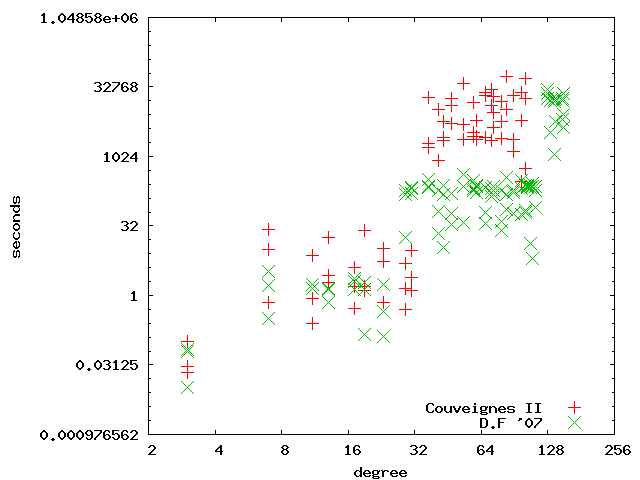
\includegraphics[width=\textwidth]{5}

      \smallskip
      \footnotesize
      \centering
      \begin{tabular}{|l|r|r|}
        \hline
        & [Cou'96] & \cite{DF07}\\
        \hline
        
        Total time           &  $65951$ & $19864$\\
        Compute $E[p^k]$    &           $0,06$\% & $0,5$\%\\
        Compute $E'[p^k]$   &             $28$\% & $89,5$\%\\
        Interpolation &             $71$\% & $9,5$\%\\
        \hline
      \end{tabular}
    \end{column}
  \end{columns}
\end{frame}

%%

\begin{frame}
  \frametitle{Timings}

  
  \begin{columns}
    \begin{column}{0.4\textwidth}
      \begin{itemize}
      \item \texttt{NTL} implemantation of \cite{DFS09} vs.  \texttt{Magma}
        implementation, of \cite{Couveignes00}
      \item $\K = \F_{2^{101}}$.
      \end{itemize}
    \end{column}
    \begin{column}{0.6\textwidth}
      \alt<2>{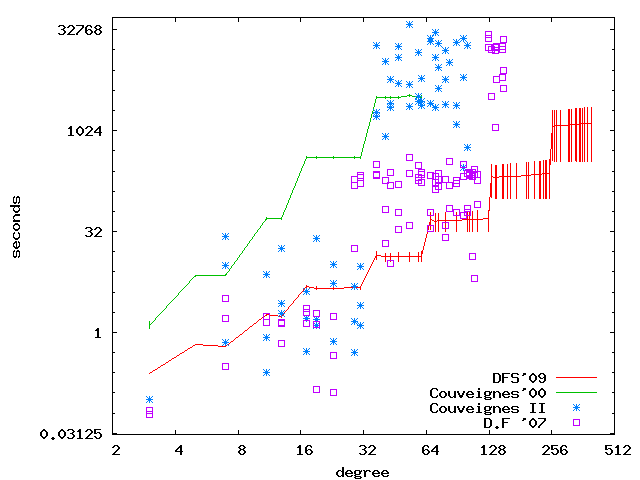
\includegraphics[width=\textwidth]{5+2-101}}
             {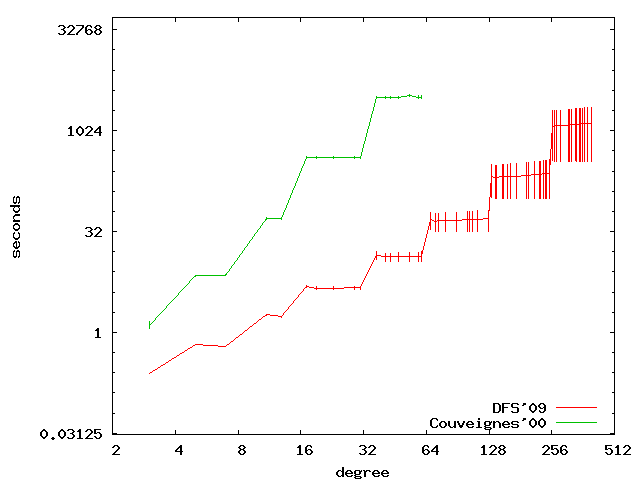
\includegraphics[width=\textwidth]{2-101}}

    \end{column}
  \end{columns}
  
  \smallskip
  \footnotesize
  \centering
  \begin{tabular}{r r r r r r r r}
    \hline
    $\ell$ & $E[p^k]$ & $E'[p^k]$ & Interp & Step 6 & ModComp & Avg tries & Avg loop time\\
    \hline
    31 & 1.3128 & 1.3128 & 1.1058 & 0.00218 & 0.00218 & 64 & 0.279\\
    61 & 3.5454 & 3.5464 & 2.5236 & 0.00783 & 0.00900 & 128 & 2.154 \\
    127 & 9.2975 & 9.3026 & 5.6881 & 0.03147 & 0.03634 & 256 & 17.359 \\
    251	& 23.7984 & 23.7984 & 12.7251 & 0.12415 & 0.14519 & 512 & 137.902 \\
    397 & 59.7439 & 59.7579 & 28.3387 & 0.36822 & 0.58027 & 1024 & 971.254 \\
    \hline
  \end{tabular}
\end{frame}

%%

\begin{frame}
  \frametitle{Timings}

  
  \begin{columns}
    \begin{column}{0.4\textwidth}
      \begin{itemize}
      \item \texttt{NTL} implemantation of \cite{DFS09}
      \item $\K = \F_{3^{64}}$.
      \end{itemize}
    \end{column}
    \begin{column}{0.6\textwidth}
      \alt<2>{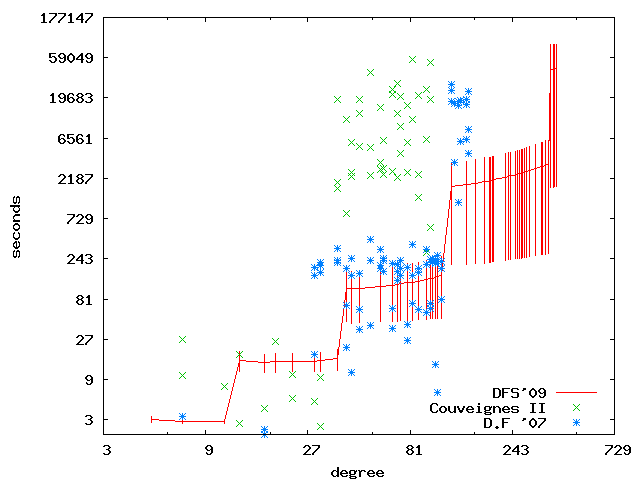
\includegraphics[width=\textwidth]{5+3-64}}
             {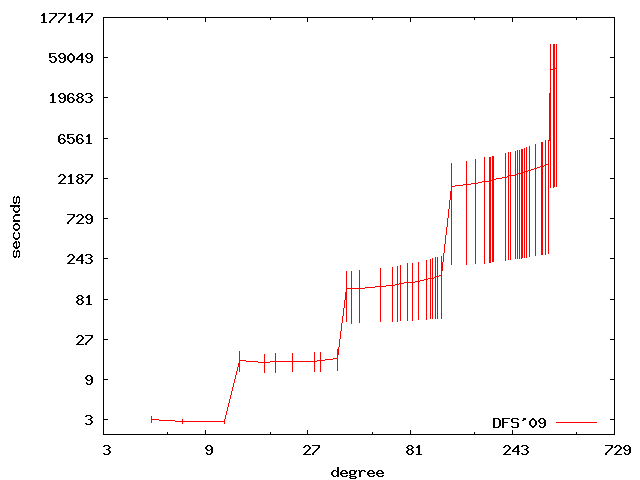
\includegraphics[width=\textwidth]{3-64}}

    \end{column}
  \end{columns}
  
  \smallskip
  \footnotesize
  \centering
  \begin{tabular}{r r r r r r r r}
    \hline
    $\ell$ & $E[p^k]$ & $E'[p^k]$ & Interp & Step 6 & ModComp & Avg tries & Avg loop time\\
    \hline
    11 & 0.6109 & 0.6109 & 0.4669 & 0.0194 & 0.0249 & 13 & 0.58 \\
    37 & 2.3946 & 2.3916 & 2.1066 & 0.1988 & 0.1381 & 40 & 13.48 \\
    113 & 9.8045 & 9.8055 & 8.5377 & 1.7712 & 0.8690 & 121 & 319.47 \\
    359 & 38.3292 & 38.3972 & 34.7147 & 17.5004 & 7.0088 & 364 & 8921.35 \\ 
    389 & 159.8280 & 159.5690 & 147.741 & 45.1558 & 69.9133 & 1093 & 125770.52  \\   
    \hline
  \end{tabular}
\end{frame}

%%

\begin{frame}
  \frametitle{Record Timings!}

  
  \begin{columns}
    \begin{column}{0.4\textwidth}
      \begin{itemize}
      \item \texttt{NTL} implemantation of \cite{DFS09}
      \item $\K = \F_{2^{1023}}$.
      \end{itemize}
    \end{column}
    \begin{column}{0.6\textwidth}
      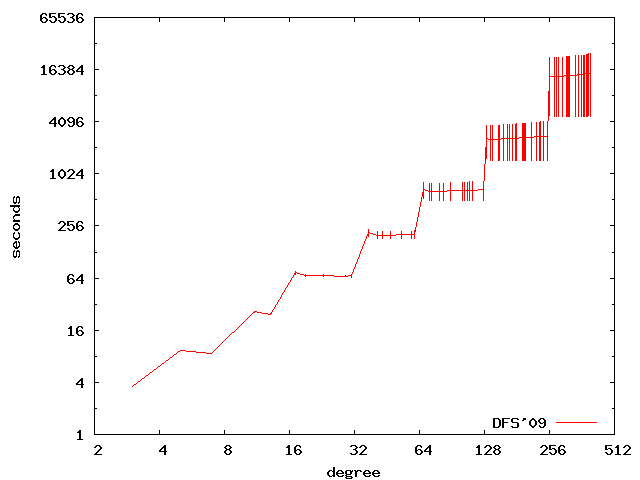
\includegraphics[width=\textwidth]{2-1023}

    \end{column}
  \end{columns}
  
  \smallskip
  \footnotesize
  \centering
  \begin{tabular}{r r r r r r r r}
    \hline
    $\ell$ & $E[p^k]$ & $E'[p^k]$ & Interp & Step 6 & ModComp & Avg tries & Avg loop time\\
    \hline
    31 & 21.182 & 21.174 & 11.597 & 0.0178 & 0.02541 & 64 & 2.768 \\
    61 & 58.656 & 58.665 & 26.826 & 0.0645 & 0.10398 & 128 & 21.576 \\
    127 & 154.357 & 154.296 & 61.202 & 0.2580 & 0.41578 & 256 & 172.503 \\
    251 & 383.773 & 383.861 & 138.428 & 0.9950 & 1.66120 & 512 & 1360.000 \\
    397 & 931.022 & 931.610 & 313.609 & 3.1819 & 6.73608 & 1024 & 10156.011 \\
    \hline
  \end{tabular}
\end{frame}

%%

\begin{frame}
  \frametitle{Ongoing work}

  \begin{block}{Implementation (with F. Morain and E. Schost)}
    \begin{itemize}
    \item \texttt{SAGE} porting of \texttt{FAAST},
    \item \texttt{SAGE} porting of SEA + Lercier + Couveignes II,
    \item comparison with Lercier,
    \item comparison with Lercier-Sirvent.
    \end{itemize}
  \end{block}

  \begin{block}{Theory}
    \begin{itemize}
    \item Try a $p$-adic version of Couveignes II + BMSS08 to reduce
      the number of tries in the final loop,
    \item Improve Lercier-Sirvent and make it the best algorithm for
      this problem.
    \end{itemize}
  \end{block}
\end{frame}

%%

\begin{frame}
  \begin{center}
    \Large
    \textbf{Thanks}
  \end{center}
\end{frame}

%%
%%

\begin{frame}
  \frametitle{Bibliography}

  \begin{thebibliography}{1}
    \beamertemplatebookbibitems
    
  \bibitem[BSS1]{BSS1} I.~Blake, G.~Seroussi \& N.~Smart
    \newblock \emph{Elliptic Curves in Cryptography}
    \newblock LMS 265, Cambridge University Press, 1999
    
  \bibitem[BSS2]{BSS2} (edited by) I.~Blake, G.~Seroussi \& N.~Smart
    \newblock \emph{Advances in Elliptic Curve Cryptography}
    \newblock LMS 317, Cambridge University Press, 2005
        
  \bibitem[Mil]{MIL} J.S.~Milne.
    \newblock \emph{Elliptic curves}.
    \newblock BookSurge Publishers, ISBN 1-4196-5257-5, 2006.

  \bibitem[Sil]{SIL1} J.H.~Silverman
    \newblock \emph{The Arithmetic of Elliptic Curves}
    \newblock GTM 106, Springer-Verlag, 1986
        
  \end{thebibliography}
\end{frame}

\begin{frame}
  \frametitle{Bibliography}

  \begin{thebibliography}{1}
    \beamertemplatearticlebibitems
    
  \bibitem[Bostan, Morain, Salvy, Schost 08]{BoMoSaSc08} A.~Bostan,
    F.~Morain, B.~Salvy, É.~Schost.  \newblock Fast algorithms for
    computing isogenies between elliptic curves.
    \newblock \emph{Math. Comp.} 77, 263, 1755-1778, 2008.
    
  \bibitem[Charles, Lauter, Goren '09]{CLG09}
    D.X.~Charles, K.E.~Lauter \& E.Z.~Goren.
    \newblock Cryptographic Hash Functions from Expander Graphs.
    \newblock \emph{J. Cryptology} 22:93--113, 2009.
    
  \bibitem[Couveignes '96]{Cou96}J.-M.~Couveignes.
    \newblock Computing $\ell$-isogenies with the $p$-torsion.
    \newblock \emph{Lecture Notes in Computer Science} vol. 1122, pages 59--65,
    Springer-Verlag, 1996.
    
  \bibitem[Couveignes '00]{Couveignes00} J.-M. Couveignes.
    \newblock Isomorphisms between {A}rtin-{S}chreier tower.
    \newblock \emph{Math. Comp.} 69(232): 1625--1631, 2000.

  \bibitem[D.F. '07]{DF07} L.~De~Feo.  \newblock Calcul d'isogénies.
    \newblock Master
    thesis. \url{http://www.lix.polytechnique.fr/Labo/Luca.De-Feo/}

  \end{thebibliography}
\end{frame}


\begin{frame}
  \frametitle{Bibliography}

  \begin{thebibliography}{1}

  \bibitem[D.F., Schost '09]{DFS09} L.~De~Feo \& É.~Schost.  \newblock
    Fast arithmetics in Artin-Schreier towers over finite fields.
    \newblock \emph{Preprint}, 2009.

  \bibitem[Gallant, Lambert, Vanstone '01]{GLV}
    R.P.~Gallant, R.J.~Lambert \& S.A.~Vanstone.
    \newblock Faster Point Multiplication on Elliptic Curves
    with Efficient Endomorphisms.
    \newblock \emph{CRYPTO '01}, LNCS, pages 190--200, Springer, 2001.
    
  \bibitem[Gaudry, Hess, Smart '02]{GHS}
    P.~Gaudry, F.~Hess, N.~P.~Smart.
    \newblock Constructive and destructive facets of Weil
    descent on elliptic curves.
    \newblock \emph{J. Cryptology} 15:19-46, 2002.

  \bibitem[Jao, Miller, Venkatesan '05]{JMV05}
    D.~Jao, S.D.~Miller \& R.~Venkatesan,
    \newblock Do All Elliptic Curves of the Same Order Have the Same 
    Difficulty of Discrete Log?
    \newblock \emph{ASIACRYPT '05}, LNCS, pages 21--40, Springer, 2005.

  \end{thebibliography}
\end{frame}

\begin{frame}
  \frametitle{Bibliography}

  \begin{thebibliography}{1}

  \bibitem[Joux, Lercier '06]{JL06}A.~Joux, R. Lercier.
    \newblock Counting points on elliptic curves in medium characteristic.
    \newblock \emph{Cryptology ePrint Archive} 2006/176, 2006.

  \bibitem[Lercier, Sirvent '09]{LS09}R.~Lercier, T~.Sirvent.
    \newblock On Elkies subgroups of $\ell$-torsion points in curves
    defined over a finite field.
    \newblock To appear \emph{J. de Théorie des Nombres de Bordeaux}.

  \bibitem[Schoof '95]{Scho95} R.~Schoof. \newblock Counting points on
    elliptic curves over finite fields. \newblock \emph{J. de Théorie
      des Nombres de Bordeaux}, 7:219-254, 1995.

  \bibitem[Smith '08]{Ben} B.~Smith.  \newblock Isogenies and the
    Discrete Logarithm Problem in Jacobians of genus $3$ hyperelliptic
    curves.
    \newblock In \emph{EUROCRYPT '08}, LNCS, Springer, 2008.

  \bibitem[Teske '06]{Tes06} E.~Teske. \newblock Elliptic curve
    trapdoor system. \newblock \emph{J. Cryptology} 19:115-133, 2006.

  \end{thebibliography}
\end{frame}


\end{document}


% Local Variables:
% mode:flyspell
% ispell-local-dictionary:"british"
% End:
%

% LocalWords:  Isogeny abelian isogenies hyperelliptic supersingular Frobenius
% LocalWords:  isogenous
